
\chapter{The FIT T0+ Detector}
The Fast Interaction Trigger is a detector system that measures the fundamental experimental parameters for analyzing particle interactions in ALICE: FIT measures the location and time of interactions, as well as multiplicity and centrality. These parameters are measured using scintillators and Cherenkov detectors. T0+ is a Cherenkov detector composed of crystals and photomultipliers; it measures the location and energy of particles that pass through the crystals. When signals are detected on multiple channels of the detector within a specified time interval, they trigger a signal that initiates data acquisition on other detector systems. This is called a coincidence measurement, and is the first data required in event reconstruction. FIT T0+ (FT0) uses coincidence measurements and channel data to determine the trajectories of particles moving transverse to the beamline.

\begin{figure}[H]
    \centering
    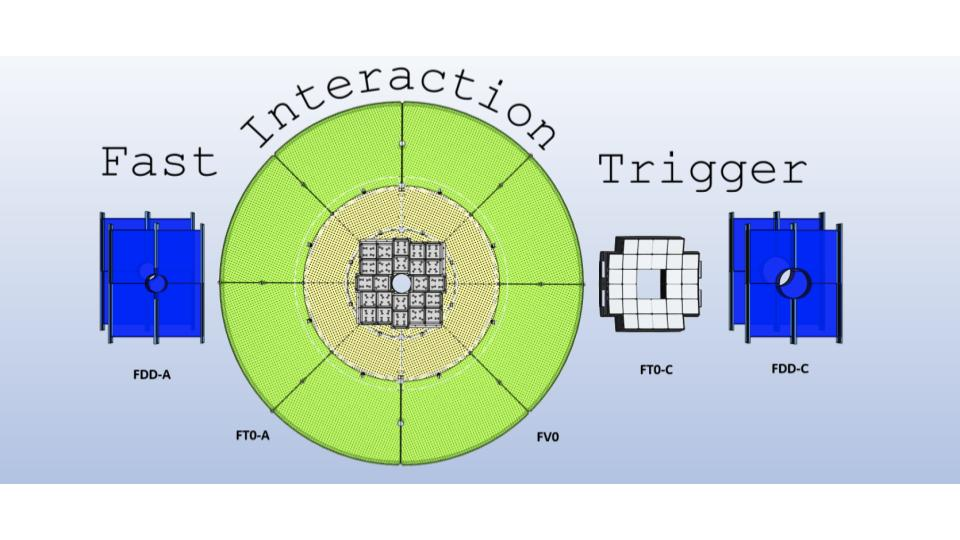
\includegraphics[width=0.6\textwidth]{figures/FIT/FIT_Logo.jpg}
    \caption{Logo for the Fast Interaction Trigger, showing the FDD, FT0, and FV0 detectors.}
    \label{fig:FIT_Logo}
\end{figure}


\section{FIT T0+ Hardware}
T0+ is a Cherenkov detector that consists of two sides, A and C. A-side and C-side sit on opposite ends of the interaction point to increase the precision of measurements on interactions that have low transverse momenta. A-side has twenty-four photomultipliers, each with four separate channels. C-side has twenty-eight photomultipliers, which are angled toward the beamline. Together, these Cherenkov detectors are used to measure important beam characteristics and trigger DAQ on other detectors in ALICE. 

\begin{figure}[H]
    \centering
    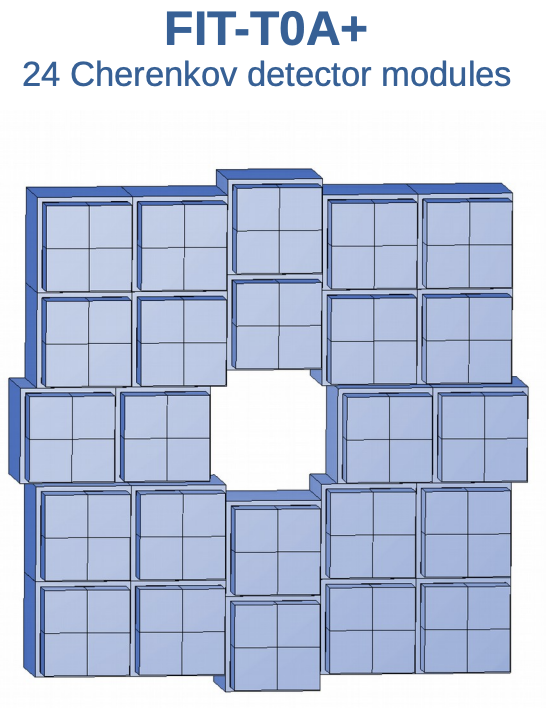
\includegraphics[width=0.4\textwidth]{figures/FIT/FT0A_Structure.png}
    \caption{Structure of the FIT T0+ A-side, with 96 channels across 24 detector modules. \cite{Slupecki}}
    \label{fig:my_label}
\end{figure}

\begin{figure}[H]
    \centering
    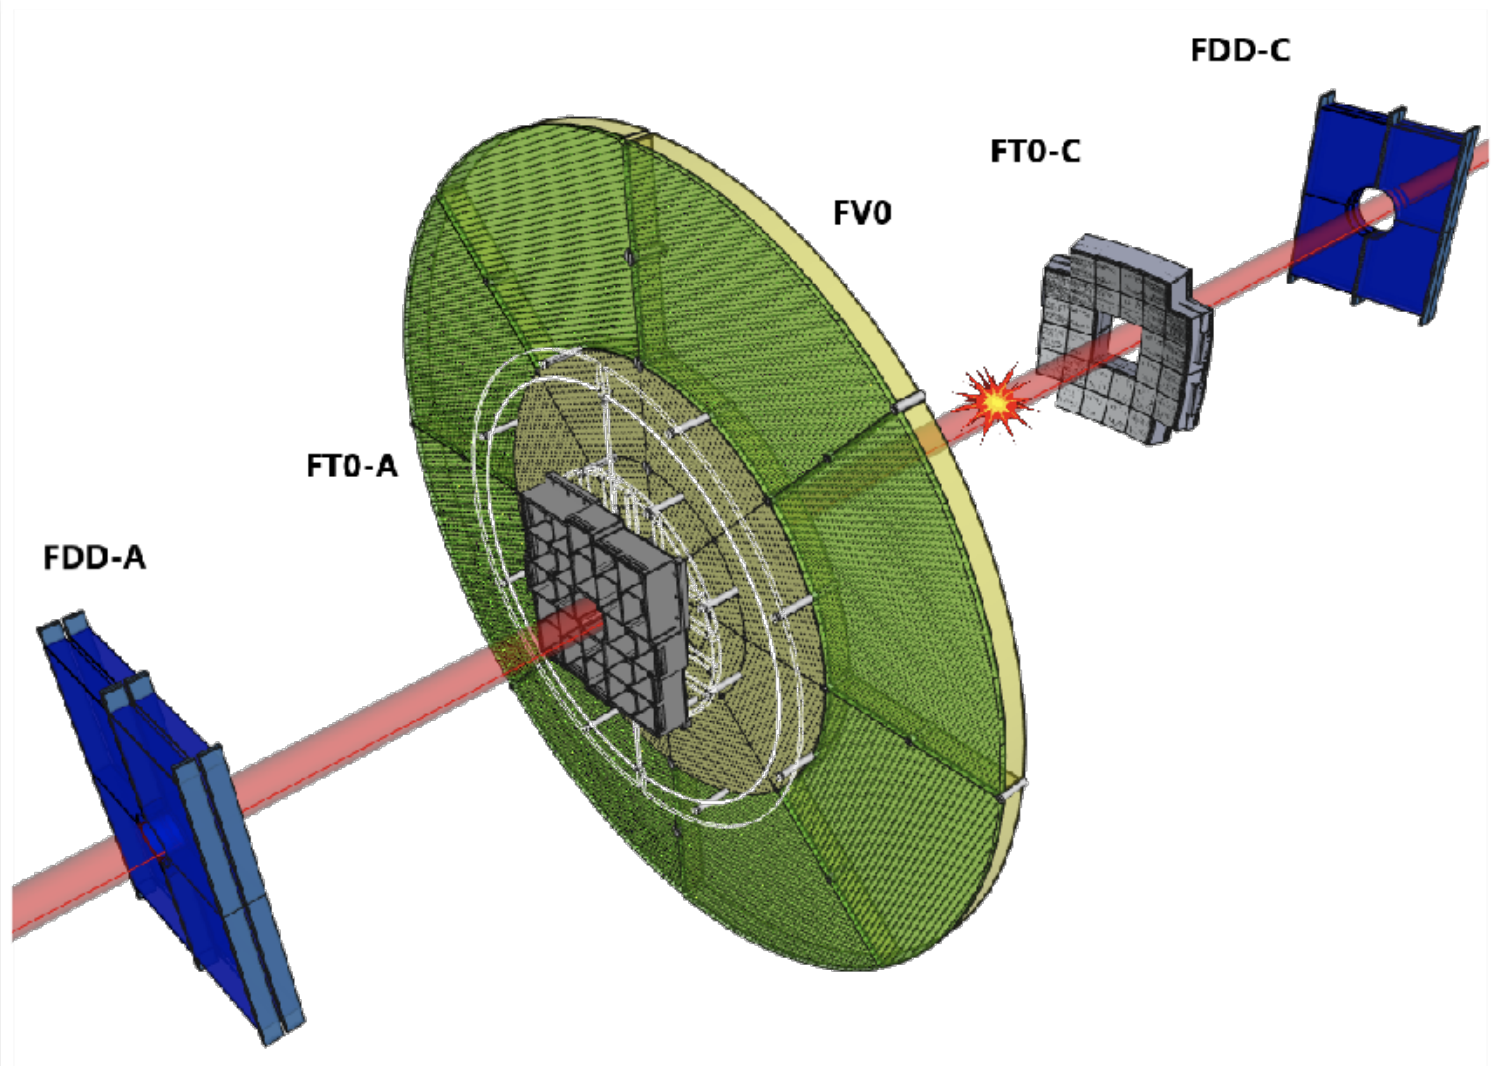
\includegraphics[width=0.6\textwidth]{figures/FIT/FIT_Layout.png}
    \caption{FIT T0+ shown in schematic view with the other detectors in FIT, V0+ and FDD. A-side and C-side are on opposite sides of the interaction point. \cite{Contreras}}
    \label{fig:FIT_Layout}
\end{figure}


\subsection{Micro-Channel Plate Photomultiplier Tube}
T0+ measures the location and energy of particles using a Cherenkov radiative quartz material coupled to a photomultiplier. Fast moving particles produce Cherenkov radiation within the quartz, which then hits the photocathode of the PMT. This produces photoelectrons that are accelerated toward metal plates called dynodes, which release more electrons. The acceleration and electron amplification is repeated across high potential differences until there are enough electrons to measure with a picoammeter. Because of this acceleration and amplification process, PMTs require high-voltage, on the order of kV. Micro-Channel Plate Photomultipliers (MCP-PMT) differ from regular photomultipliers in that they do not have discrete dynodes, instead having thin glass plates with many holes with diameter 1-100$\mu$m. MCP-PMTs are required in ALICE because of their minimal gain loss in strong magnetic fields. Having multiple anodes that read the current passing through provides better spacial resolution than the single-anode PMT. The electronics for the FIT T0 MCP-PMTs are shown in Fig. \ref{fig:MCP_PMT_Schematic}.
\begin{figure}[H]
    \centering
    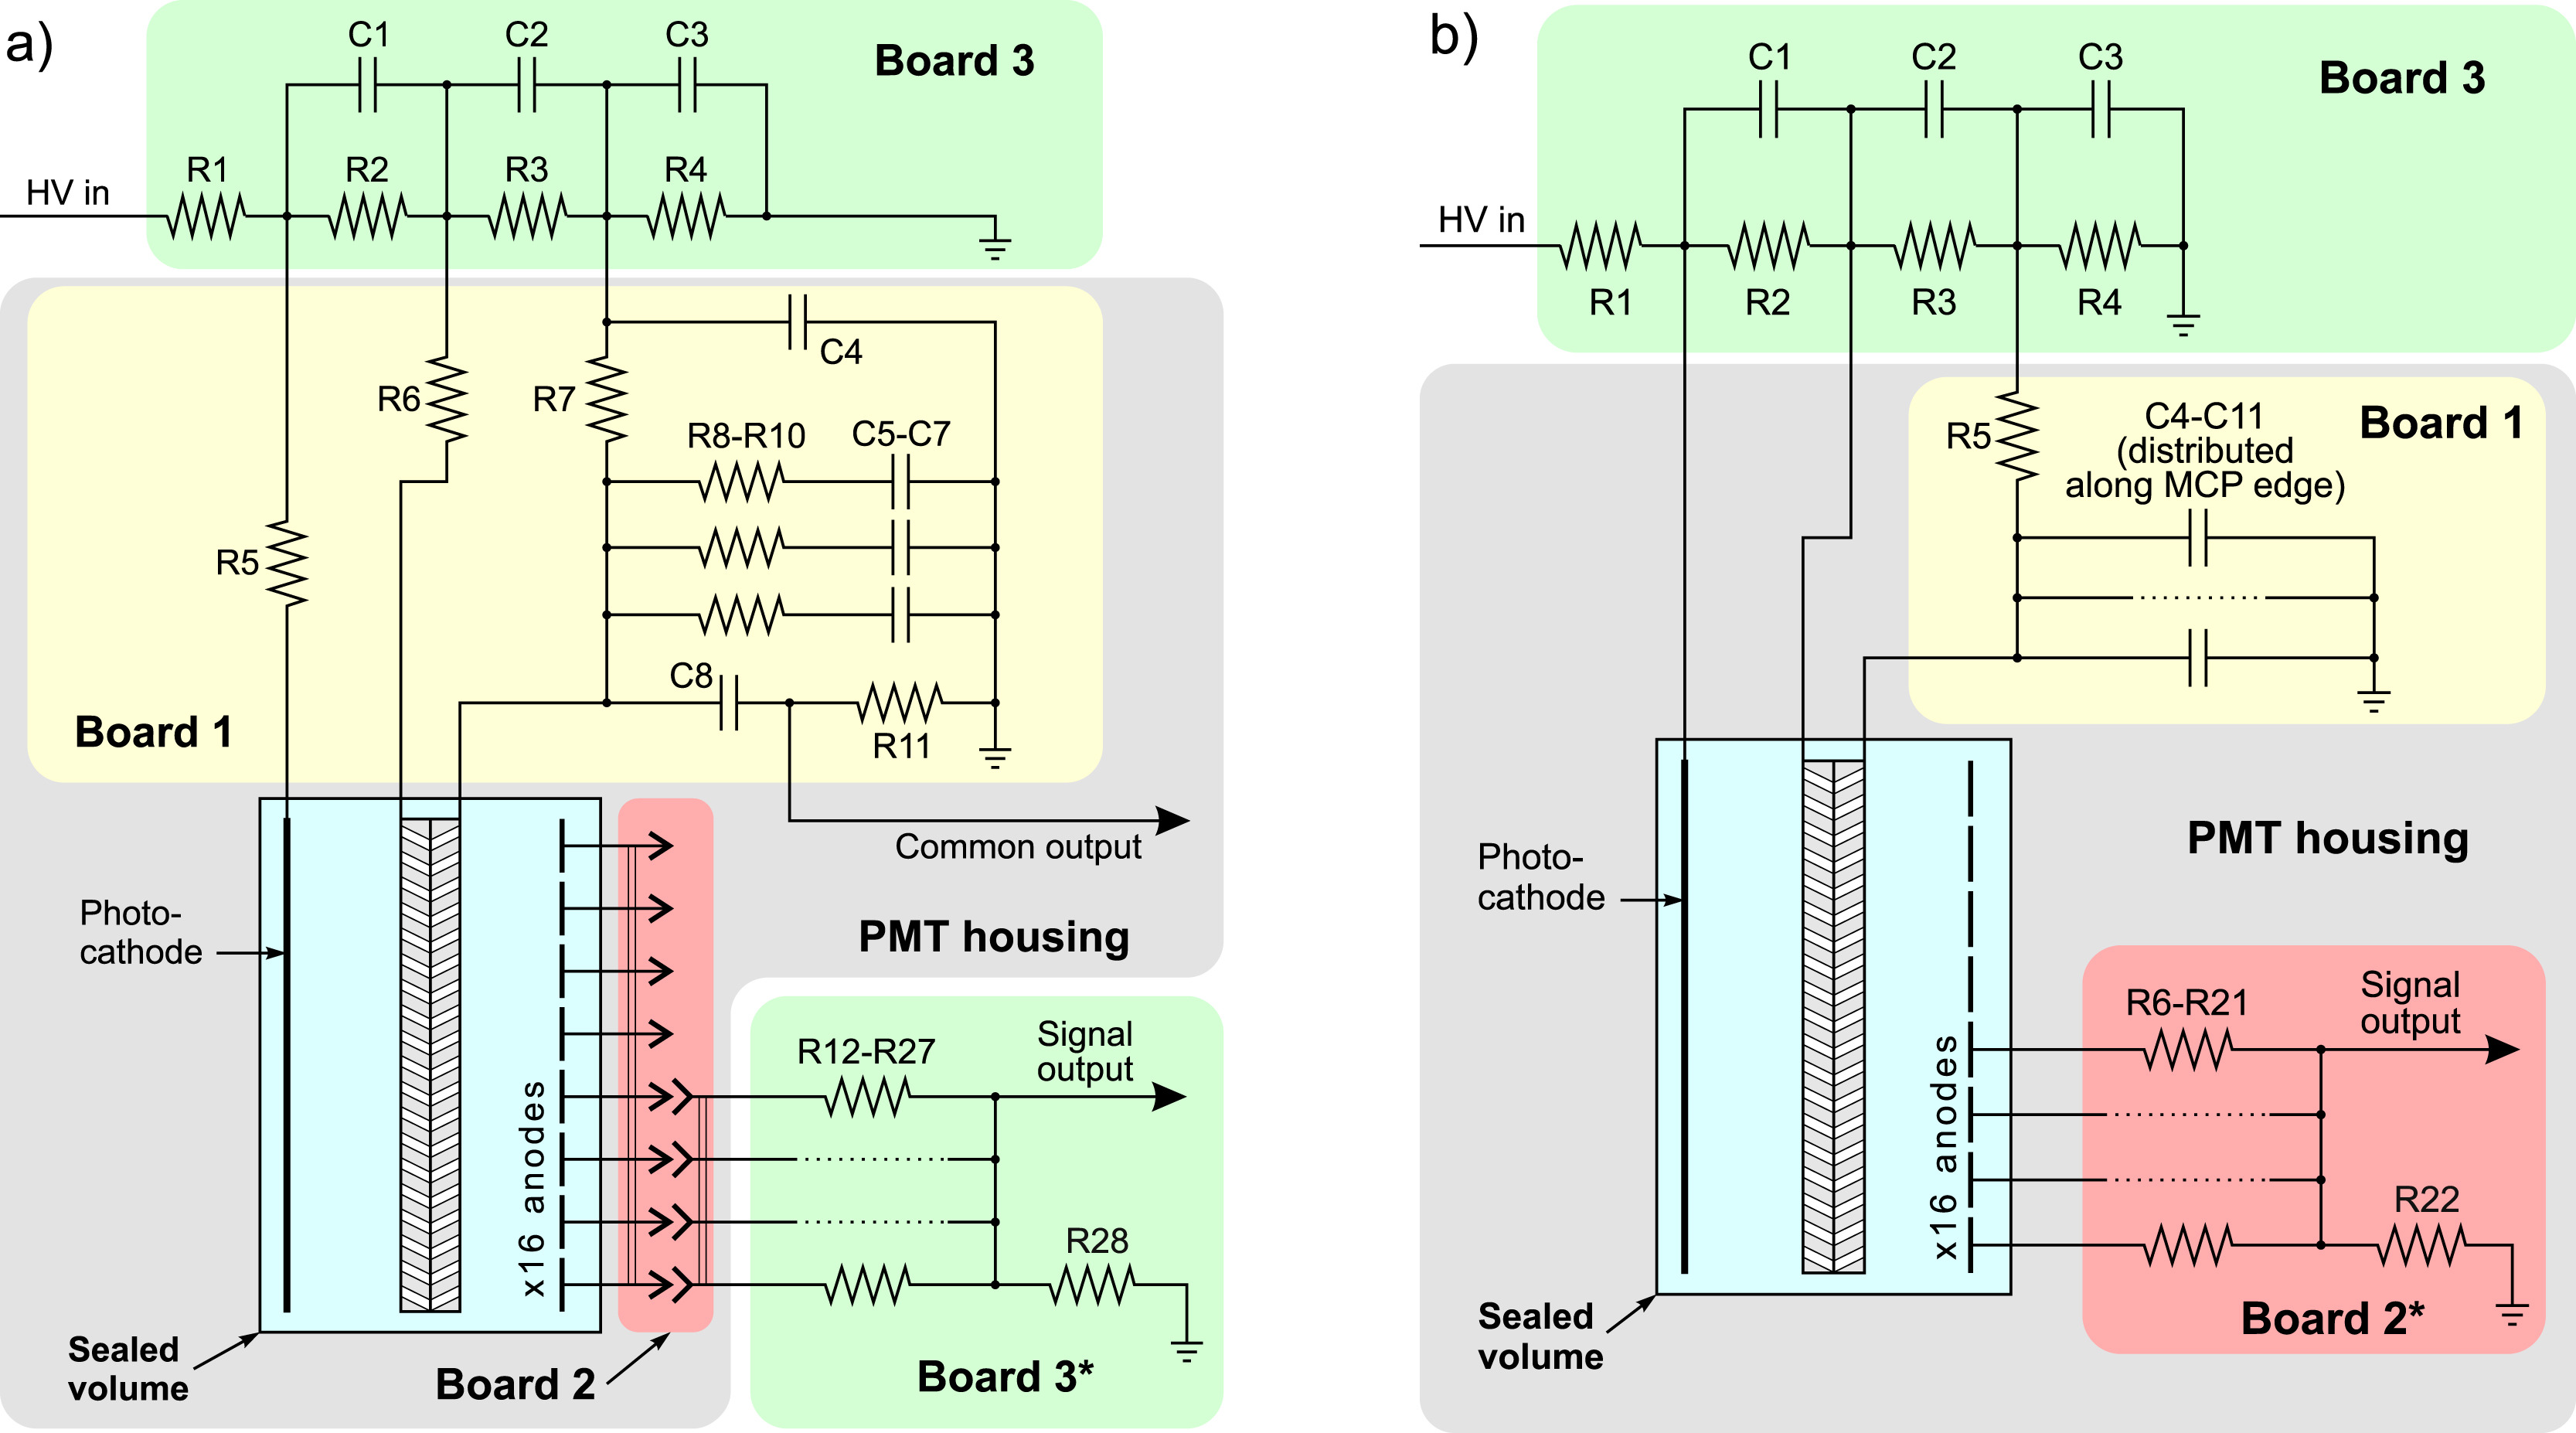
\includegraphics[width=0.8\textwidth]{figures/FIT/PMT_Schematic.jpg} 
    \caption{Schematic for the MCP-PMTs used for the FIT T0+ Cherenkov detector \cite{Yury_MCP-PMT}}
    \label{fig:MCP_PMT_Schematic}
\end{figure}



\sectionWithFixedHeader{High-Voltage Power Electronics for MCP-PMT}{HV PMT Electronics}
MCP-PMTs require large potential differences to create a measurable current from a photon that hits the photocathode. However, if the voltage is too high, then the signal can become saturated, and the resolution of the detector is compromised. Fig. \ref{fig:MCP_PMT_Schematic} shows a schematic view of the MCP-PMTs in FIT. Each PMT is equipped with a voltage divider circuit that takes in a voltage of $\sim$2 kV, and supplies voltage to three of the elements in board one: the photocathode, and on either side of the micro-channel plate. The assembly of the HV power electronics was done in summer of 2019 at the FIT lab at CERN. This includes adding coaxial LEMO connectors to the HV cables and securing the cables to the power board (Board 3 in Fig. \ref{fig:MCP_PMT_Schematic}). The assembled power electronics are shown in Fig. \ref{fig:power_board}.

\begin{figure}[H]
    \centering
    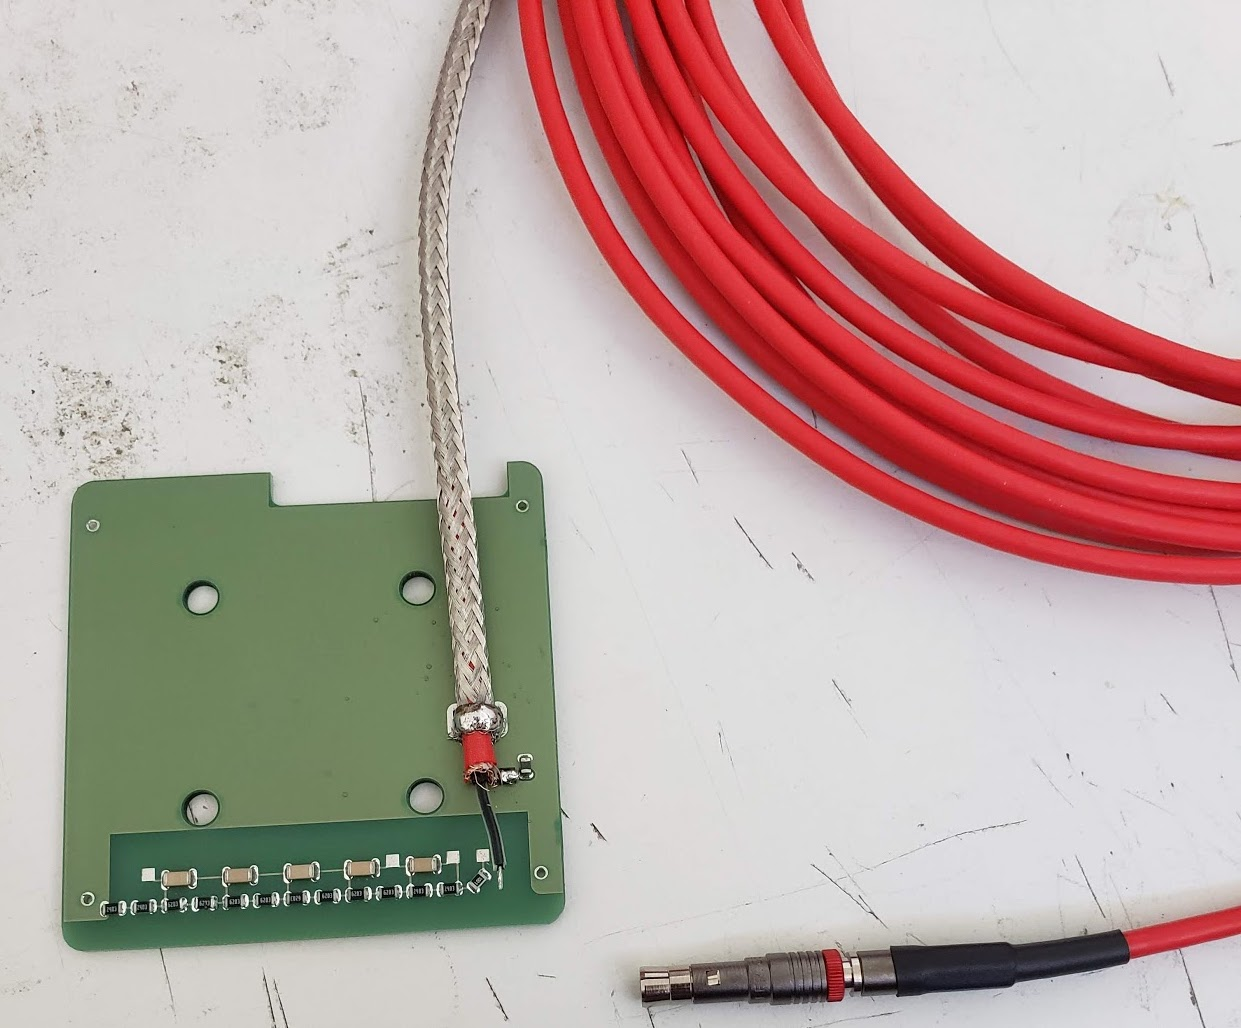
\includegraphics[width=0.6\textwidth]{figures/FIT/power_board.jpg}
    \caption{HV power electronics for MCP-PMT in FIT T0+ A-side}
    \label{fig:power_board}
\end{figure}

\section{MCP-PMT Testing at CERN}\label{pmt_testing}
During LS2, the FIT collaboration has been working on the upgrades to the hardware for T0+, hoping to increase resolution, minimize crosstalk, and maximize the trigger efficiency. This is done using the MCP-PMTs showin in Fig \ref{fig:MCP_PMT_Schematic}, which are split into four channels based on the 16 anodes. Before this hardware is installed in ALICE, it must be tested for optimal performance. To test the most important aspects of MCP-PMT performance, laser pulses are sent to the PMTs to measure the response. The pulses are produced by a laser, then split to have a reference signal. The reference signal is measured on a PMT with well known characteristics. The test signal is sent to one of the PMTs in T0+. By comparing the output current spikes from the reference and the test PMTs, we can test the performance of PMTs as they are shipped from Hamamatsu. 


\begin{figure}[H]
    \centering
    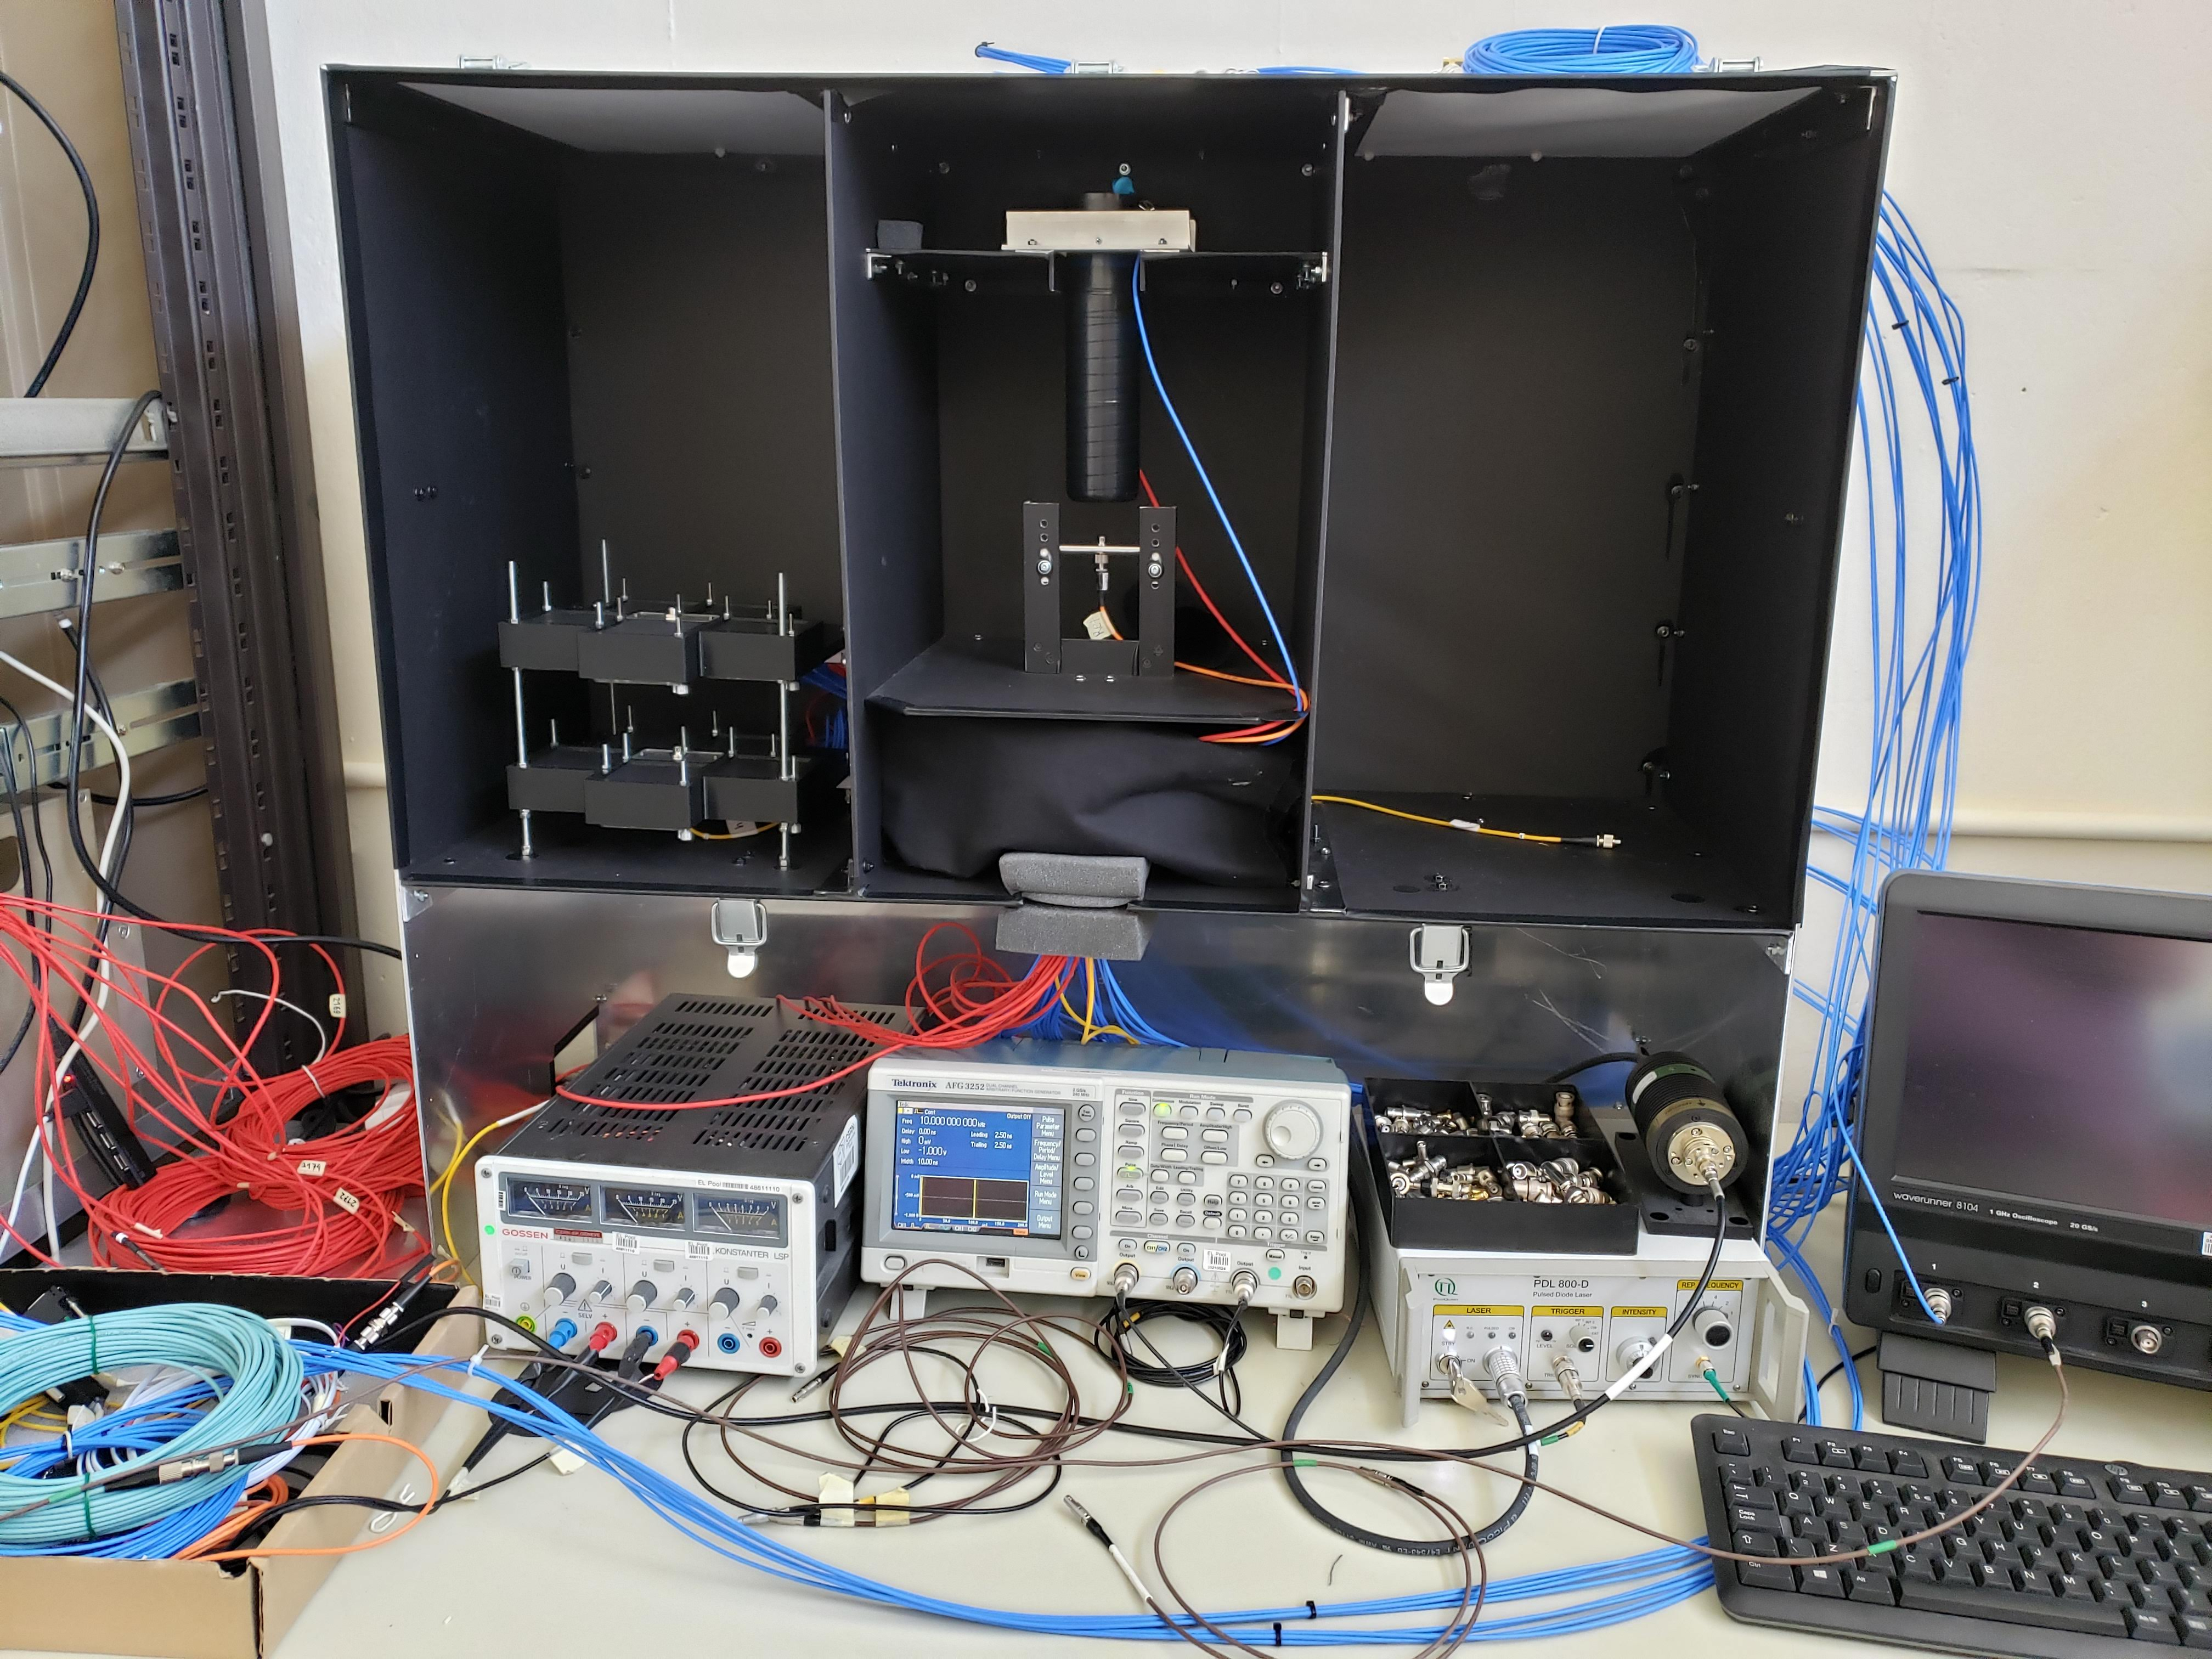
\includegraphics[width=0.8\textwidth]{figures/FIT/PMT_Test_apparatus.jpg}
    \caption{MCP-PMT Testing apparatus at the ALICE FIT Lab. Laser pulser, HV power supply, oscilloscope, function generator, isolating aluminum frame for light-tight data collection.}
    \label{fig:PMT_Testing_Apparatus}
\end{figure}

\begin{figure}[H]
  \centering
  \subfloat[T0+ C-side test assembly for MCP-PMTs in the FIT Lab.]{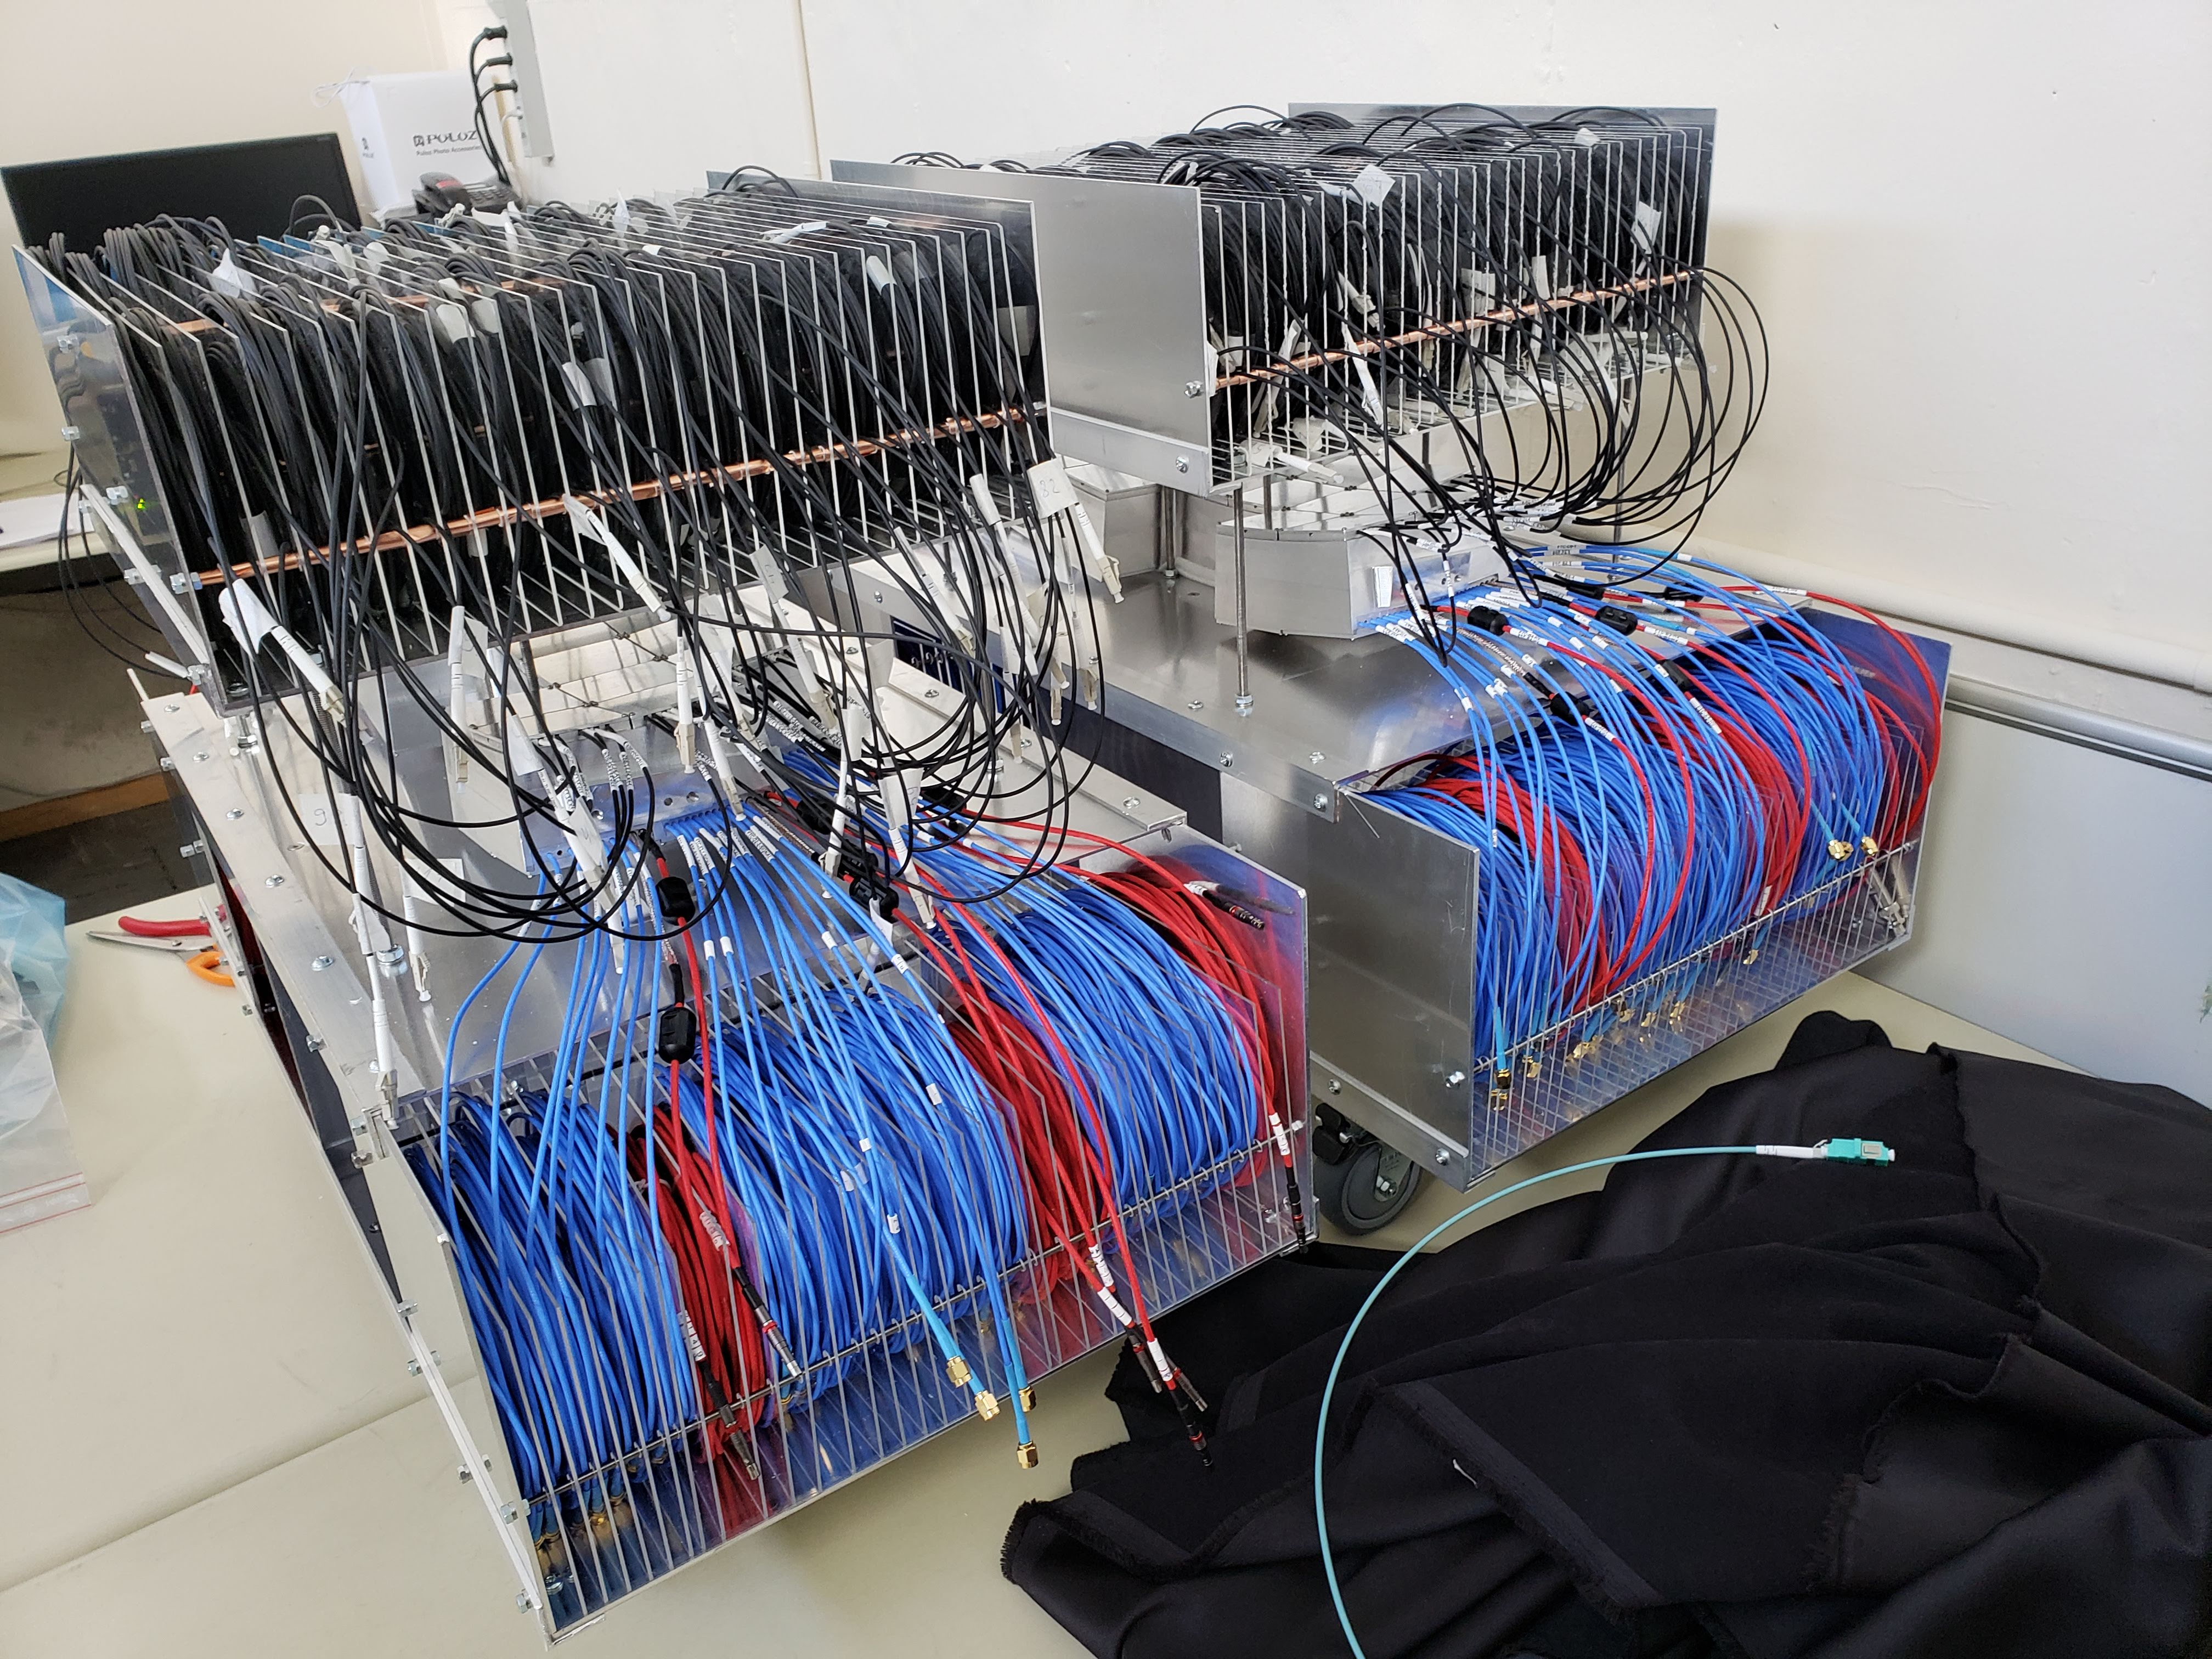
\includegraphics[width=0.4\textwidth]{figures/FIT/FT0_C_TestBench.jpg}\label{fig:FT0C_TestAssembly}}
  \hfill
  \subfloat[Side view of T0+C test assembly, showing the Aluminum support structure that holds the quartz radiators and PMTs.]{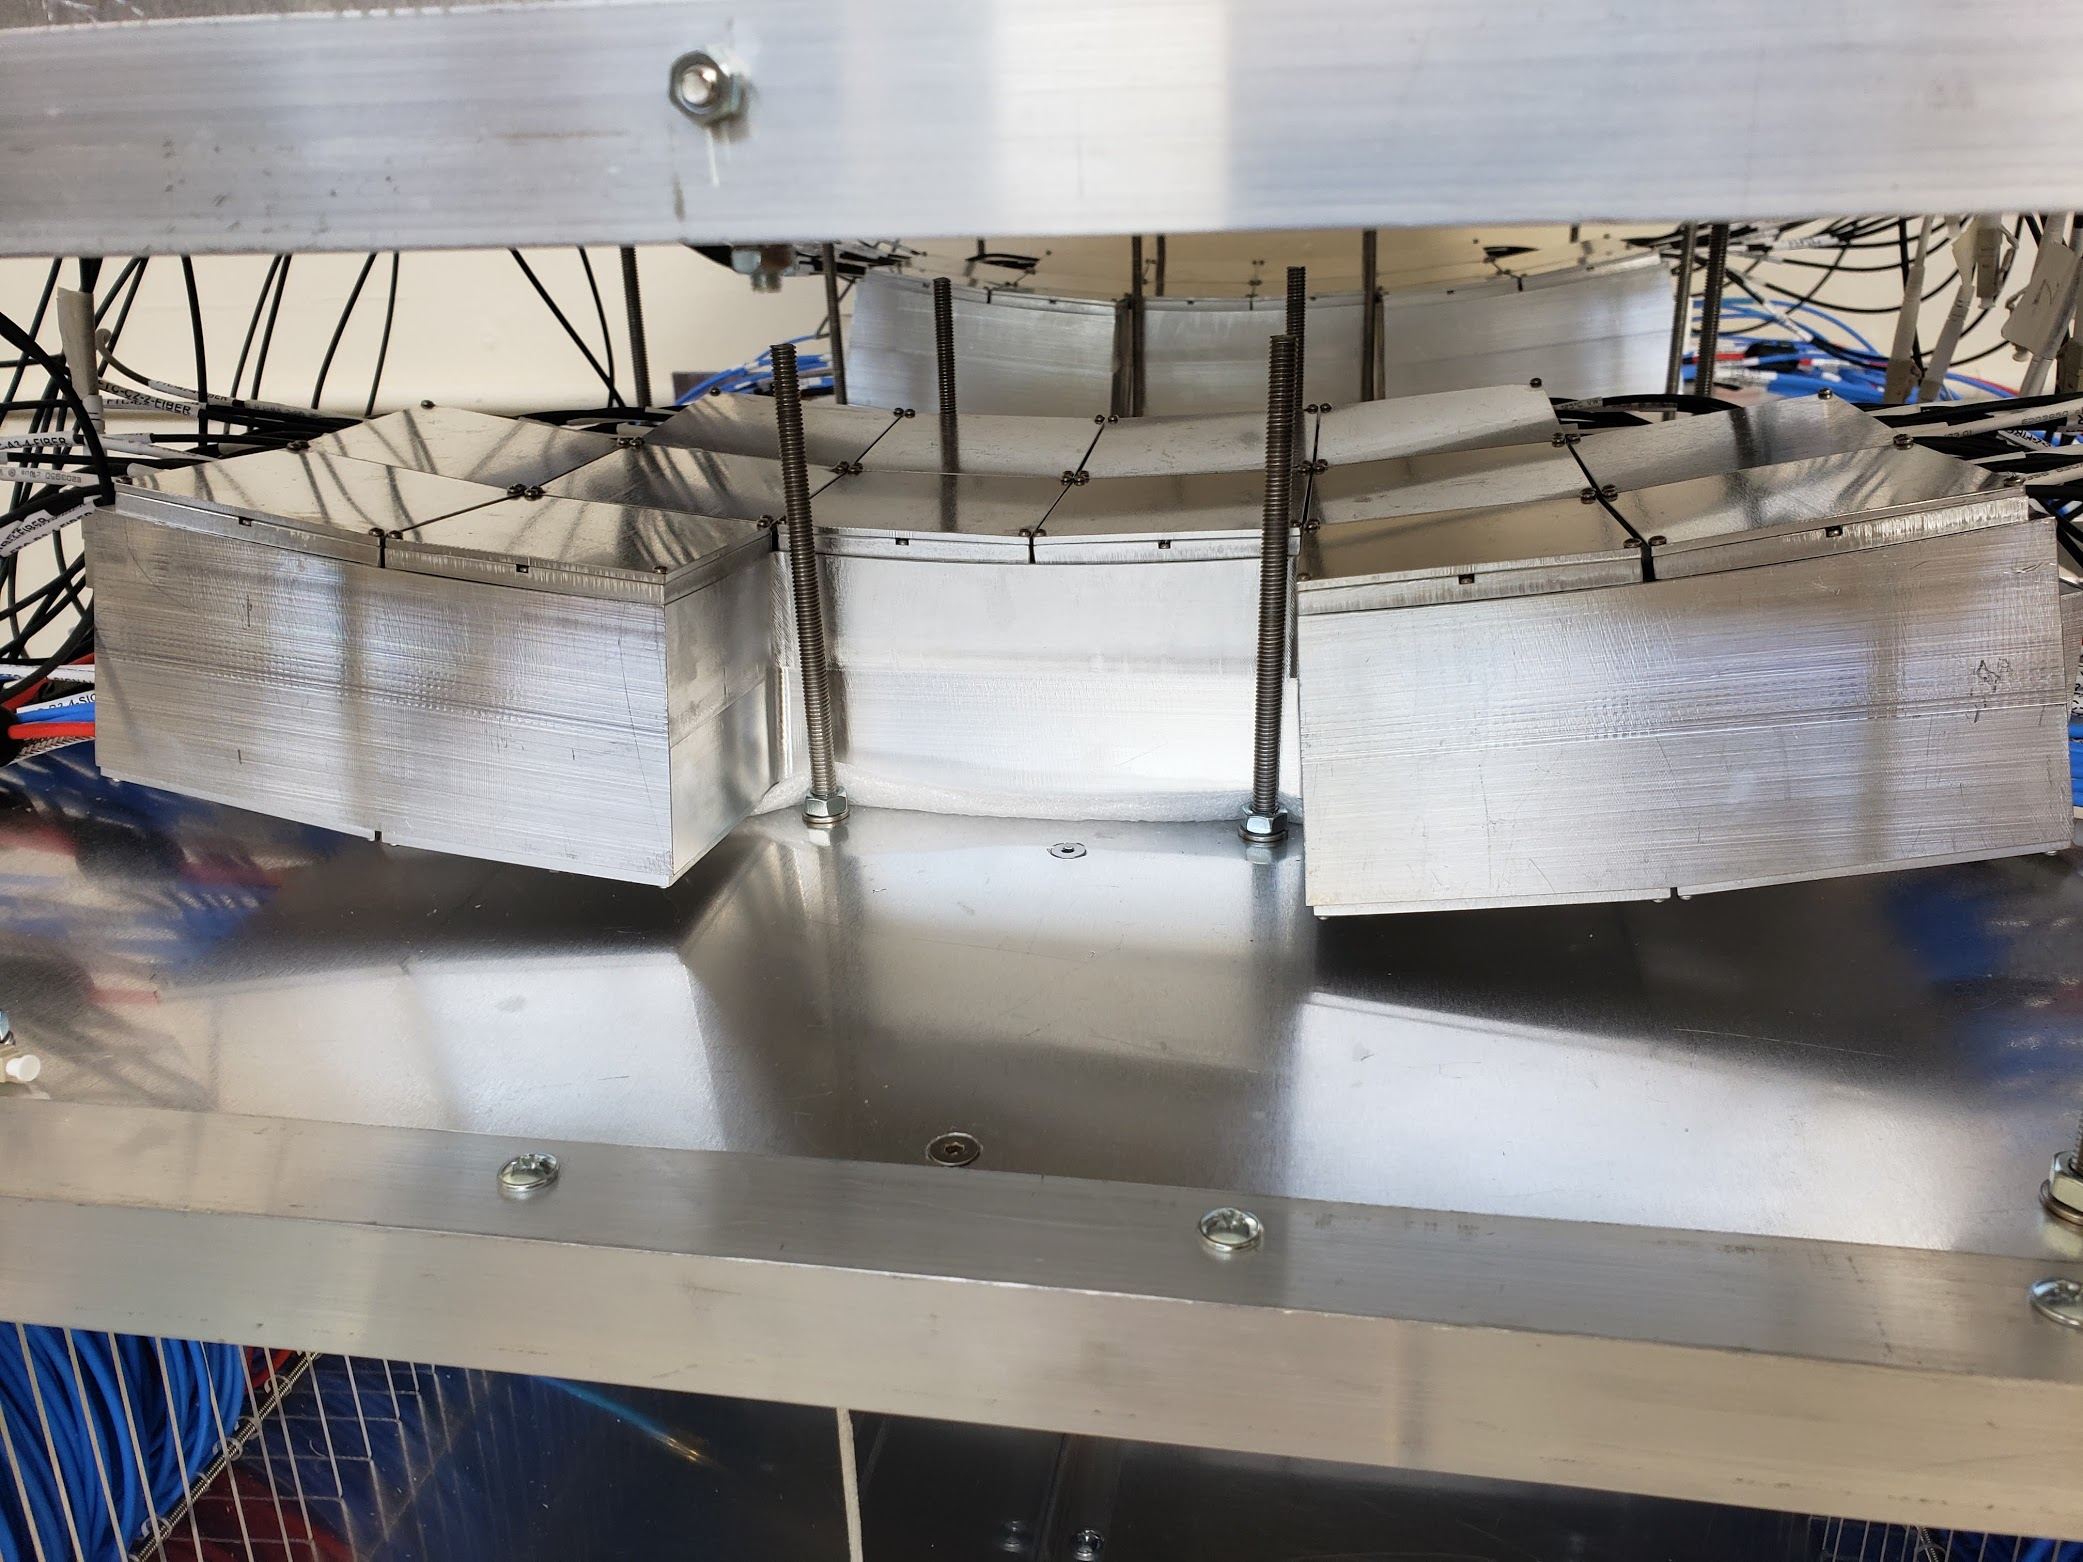
\includegraphics[width=0.4\textwidth]{figures/FIT/FT0_C_half.jpg}\label{fig:FT0C_In_Al_Structure}}
  \caption{FIT T0+ C-side in the FIT lab for MCP-PMT testing.}
\end{figure}


\begin{figure}[H]
    \centering
    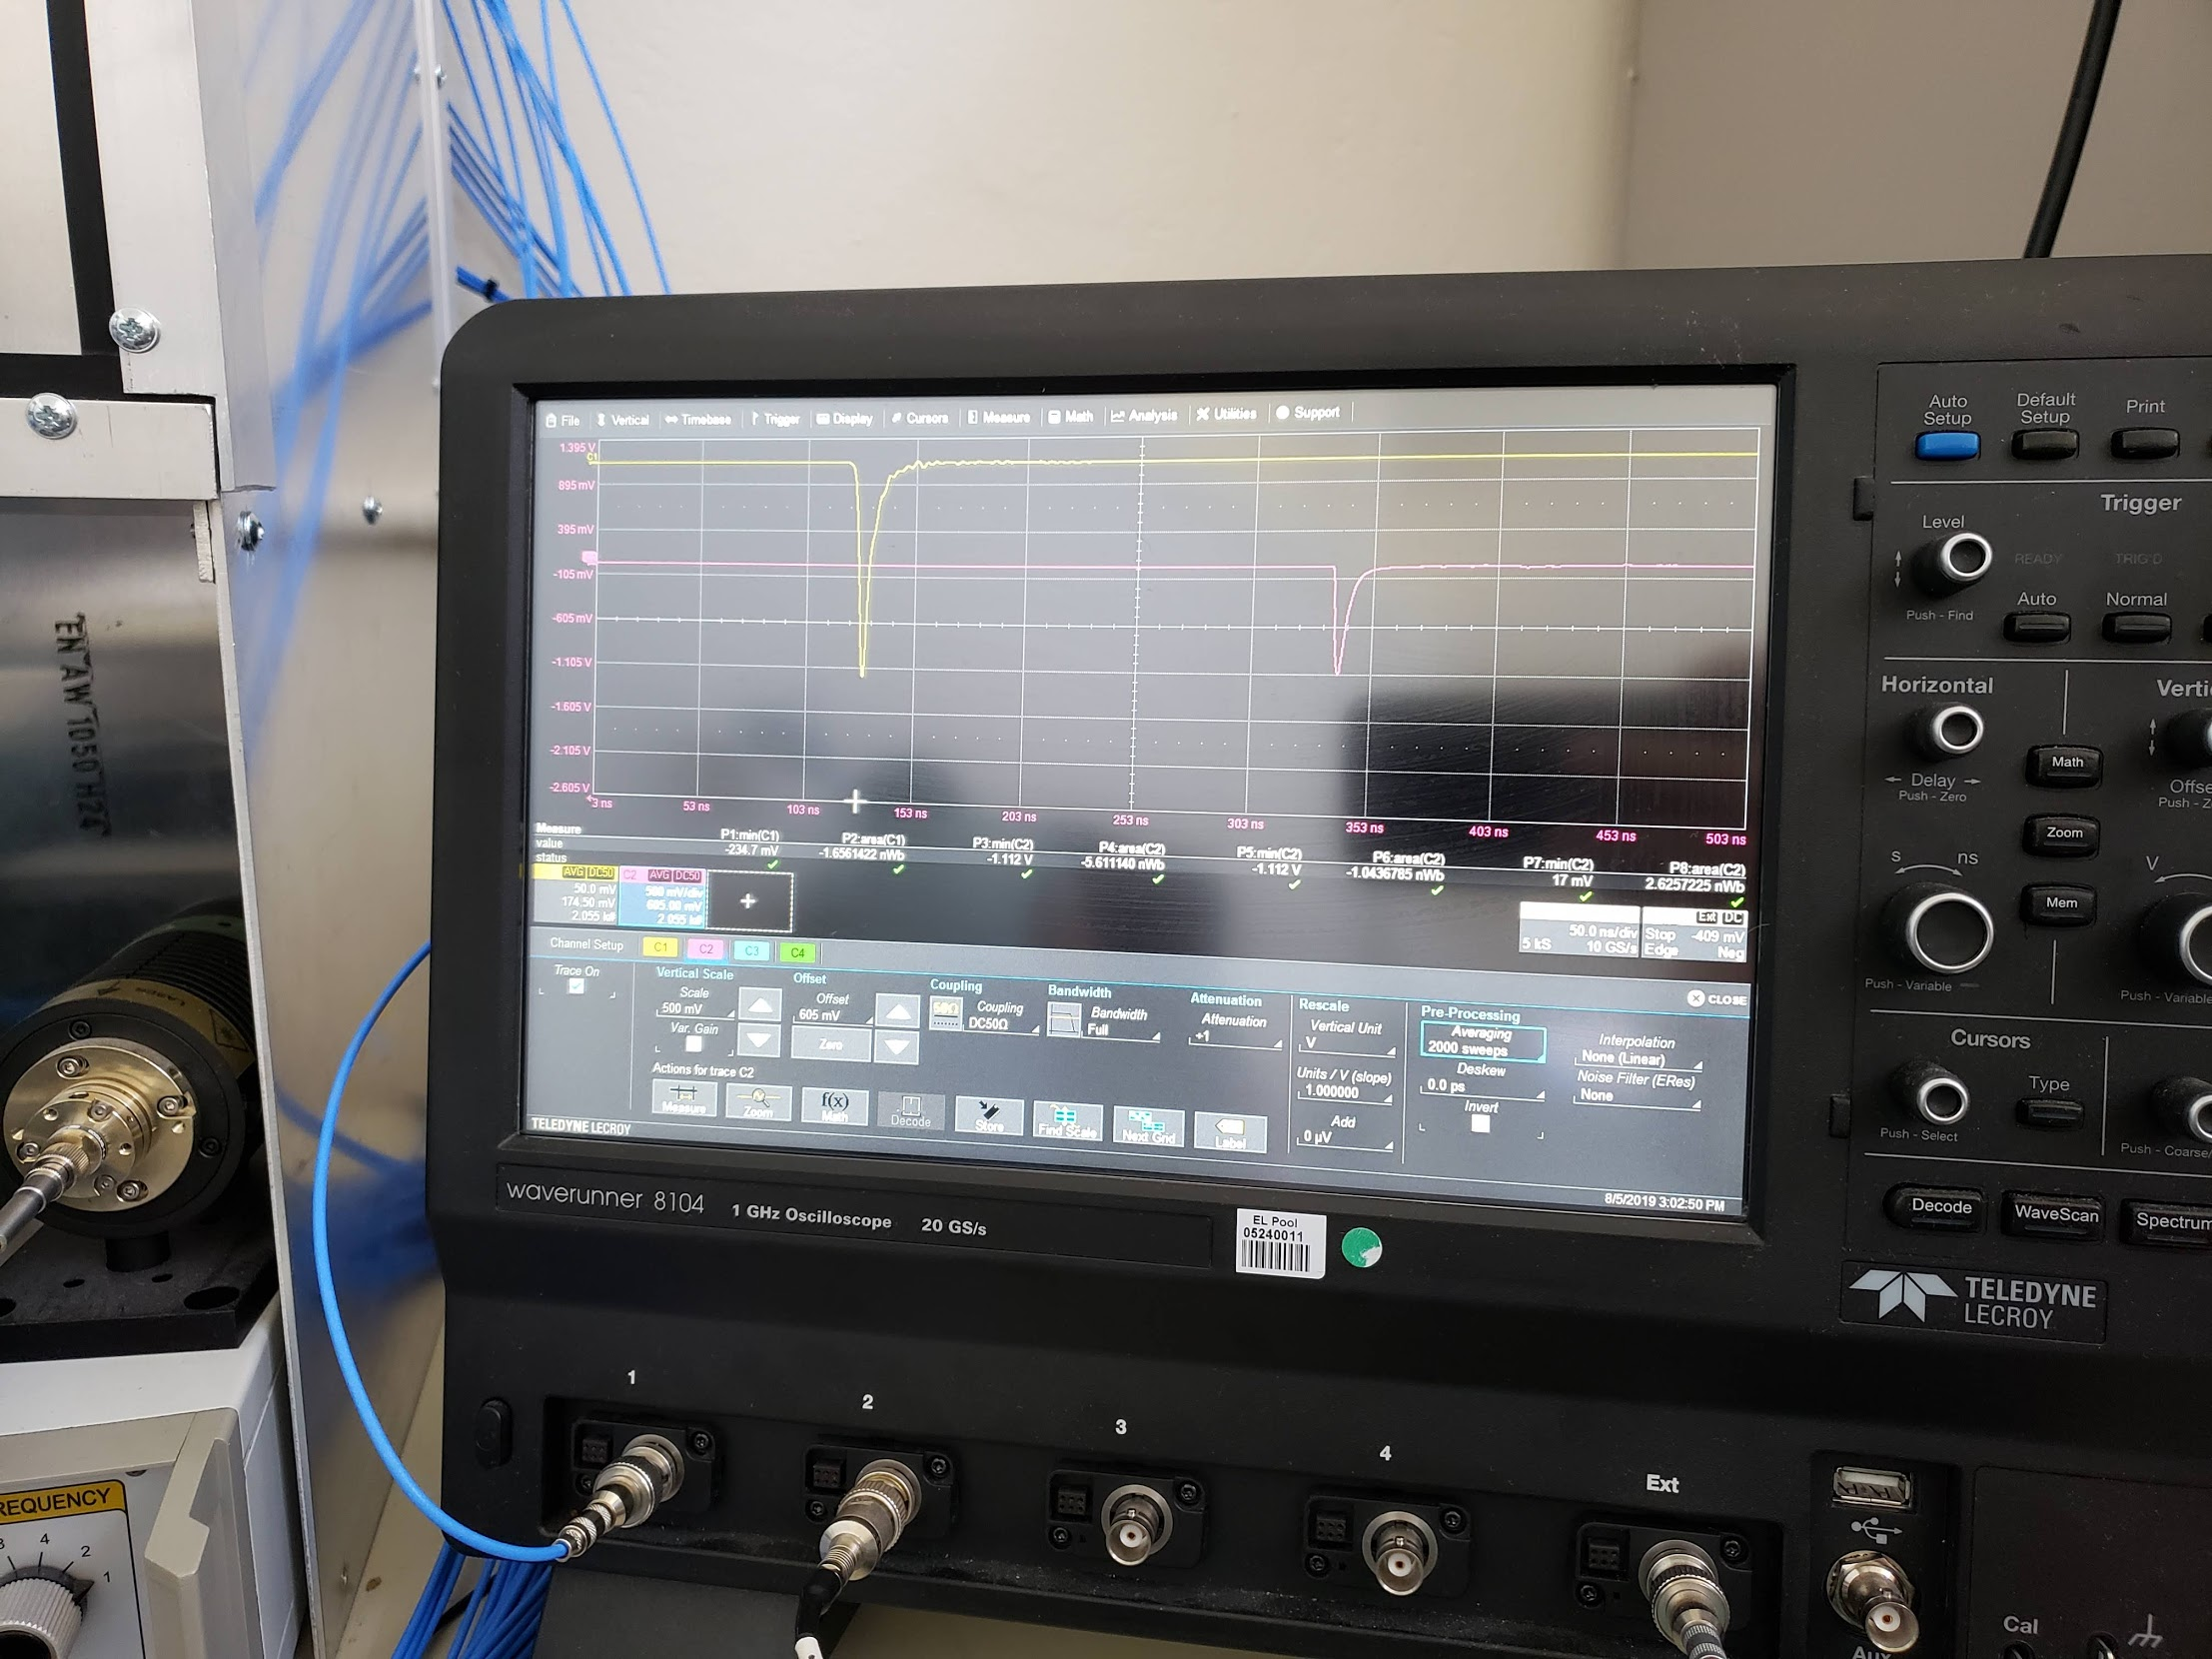
\includegraphics[width=0.8\textwidth]{figures/FIT/PMT_test_pulse.jpg}
    \caption{Oscilloscope trace of a current spike from a reference PMT (yellow) and the test PMT (pink).}
    \label{fig:my_label}
\end{figure}

